The failure rate can be translated to be in fails/year. This is done in \autoref{eq:failrate}.

\begin{flalign}
	\lambda=\frac{1 \mathrm{fails}}{2\cdot10^6\mathrm{h}}\cdot\frac{8760 \mathrm{h}}{1\mathrm{year}}=\frac{1 \mathrm{fails}}{288.3\mathrm{year}}
	\label{eq:failrate}
\end{flalign}

The lifetime of the car can be expressed by its probability density function seen in \autoref{eq:carpdf}.
\begin{flalign}
	f_{\mathrm{car}}(t)=
	\begin{cases}
		\frac{1}{10} & \text{if } t\in[5,15]\\
		0               & \text{otherwise}
	\end{cases}
	\label{eq:carpdf}
\end{flalign}
\subsection{Case 1}
For the first case, the reliability, cumulative and probability functions for the lifetime of the network can be found. The first one obtained is the reliability function and it is found by multiplying the individual reliabilities for the two switches as they are connected in series, see \autoref{fig:case1}, and they have independent probabilities of failing. 
\begin{figure}[H]
	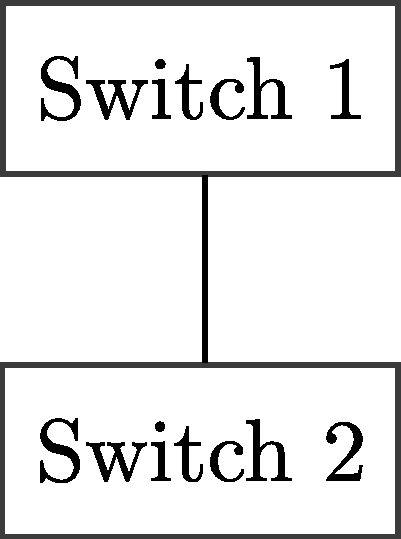
\includegraphics[width = .18\textwidth]{case1}
	\caption{Switch diagram for case 1} \label{fig:case1}
\end{figure}
%
\begin{flalign}
	R_{\mathrm{n}}(t)&=R_1(t)R_2(t)=e^{-\lambda t}e^{-\lambda t}=e^{-2\lambda  t}\label{eq:reliabilitycase1} \\
	F_{\mathrm{n}}(t)&=1-R_{\mathrm{n}}(t)=1-e^{-2\lambda t} \label{eq:cumulativecase1}  \\
	f_{\mathrm{n}}(t)&={F^{\prime}}_{\mathrm{n}}=-2 \lambda e^{{-2\lambda t}} \label{eq:probabilitycase1}  
\end{flalign}

To find the probability of the network failing before the rest of the car does, a double integration is performed from 5 to 15 for and from 0 to $t_{\mathrm{c}}$, where $t_{\mathrm{c}}$ is the time in which the car fails. \autoref{eq:integralcase1} shows the performed computation.
%
\begin{flalign}
	P(t_\mathrm{n}-t_\mathrm{c})&=\int_{5}^{15}\left[\int_{0}^{t_{\mathrm{c}}}f_{\mathrm{n}}(t)f_{\mathrm{c}}(t)dt_{\mathrm{n}}\right]dt_{\mathrm{c}}\label{eq:integralcase1}
\end{flalign}

The result of this integral gave a probability of 0.0668 of the network failing before the rest of the car.
\subsection{Case 2 a}
In case 2 a, one of the switches is duplicated as seen in \autoref{fig:case2a}. Even though the method is the same, the reliability, cumulative and probability functions change as now there is one more switch in the network. 
\begin{figure}[H]
	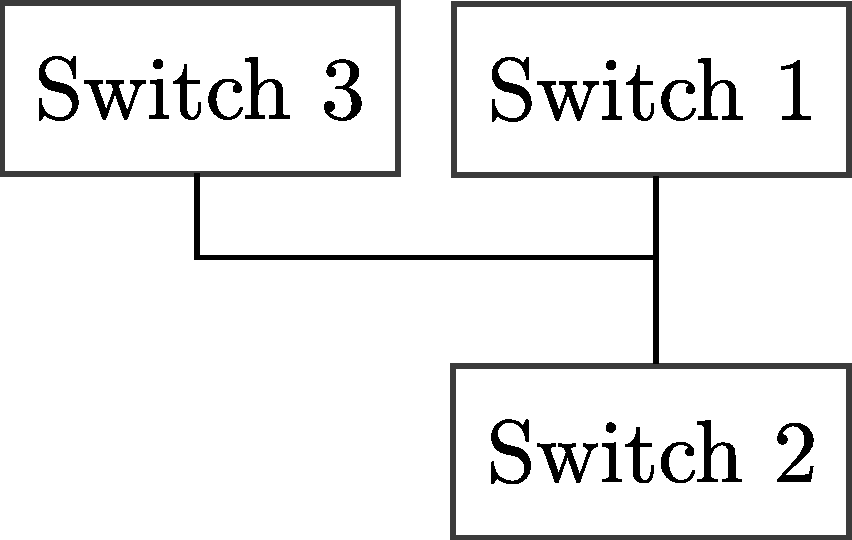
\includegraphics[width = .25\textwidth]{case2a}
	\caption{Switch diagram for case 2 a}
	\label{fig:case2a}
\end{figure}
%
\begin{flalign}
	R_{\mathrm{n}}(t)&=R_2(R_1(t)+R_3(t)-R_1(t)R_3(t))=e^{-\lambda t}\left(2e^{-\lambda t}-e^{-2\lambda  t}\right)= 2e^{-2\lambda  t} - e^{-3 \lambda t} \label{eq:reliabilitycase2a} \\
	F_{\mathrm{n}}(t)&=1-R_{\mathrm{n}}(t)= 1-2e^{-2\lambda  t} + e^{-3 \lambda t}\label{eq:cumulativecase2a}  \\
	f_{\mathrm{n}}(t)&={F^{\prime}}_{\mathrm{n}}=4 \lambda e^{{-2\lambda t}} -3 \lambda e^{{-3\lambda t}}  \label{eq:probabilitycase2a}  
\end{flalign}

The integral is done in the same way as seen in \autoref{eq:integralcase1} but in this case the expression for $f_{\mathrm{n}}$ is different. The result obtained is 0.00346.

\subsection{Case 2 b}
In the last case, both switches are duplicated. The structure is shown in \autoref{fig:case2b}. Again, the reliability, cumulative and probability functions change and they need to be re-calculated taking into account the new combination of series and parallel connection. This is shown in \autoref{eq:reliabilitycase2b} and \ref{eq:cumulativecase2b} and \ref{eq:probabilitycase2b}.
\begin{figure}[H]
	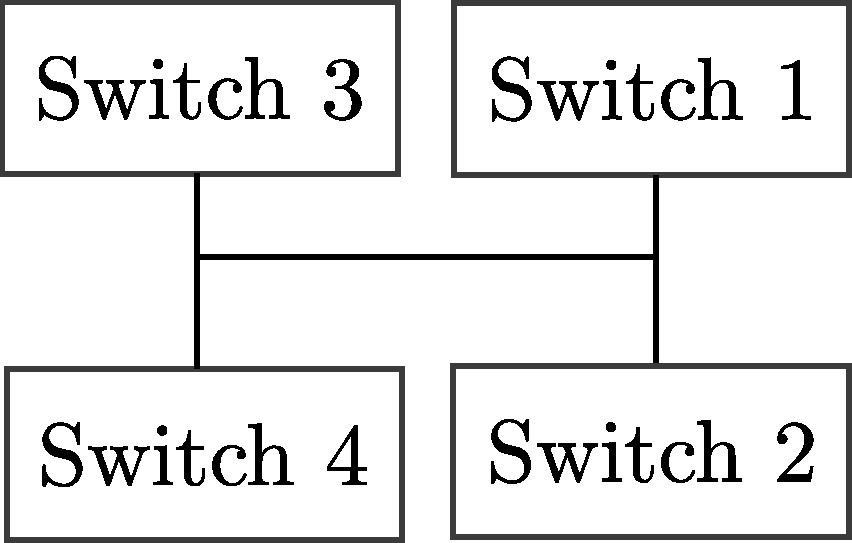
\includegraphics[width = .25\textwidth]{case2b}
	\caption{Switch diagram for case 2 b}
	\label{fig:case2b}
\end{figure}
%
\begin{flalign}
	R_{\mathrm{n}}(t)&=(R_1(t)+R_3(t)-R_1(t)R_2(t))(R_2(t)+R_4(t)-R_2(t)R_4(t))=\label{eq:reliabilitycase2b} \\
			&\left(2e^{-\lambda t}-e^{-2\lambda  t}\right)\left(2e^{-\lambda t}-e^{-2\lambda  t}\right)=\left(4e^{-2\lambda t}-4e^{-3\lambda t}+e^{-4\lambda t}\right)\nonumber\\
	F_{\mathrm{n}}(t)&=1-R_{\mathrm{n}}(t)=1-e^{-2\lambda t} \label{eq:cumulativecase2b}  \\
	f_{\mathrm{n}}(t)&={F^{\prime}}_{\mathrm{n}}=-2 \lambda e^{{-2\lambda t}} \label{eq:probabilitycase2b}  
\end{flalign}

The new probability density function is used to find the probability of the network failing before the car does in the same way as with the previous two cases. See \autoref{eq:integralcase1}. The result obtained for this case is 0.0025. 

It can be seen that the failure probability is reduces the more redundant components are present in the network.